%Section 2: Why PDAC is hard to image (biology-driven challenges).

%pancreas anatomy

The pancreas is an accesory organ of the digestive system, just like the liver, the gallbladder and salivary glands. The pancreas is located in the upper abdomen retroperitoneally, that is behind the peritoneum, the tissue that lines the abdominal wall and covers most of the abdominal organs \cite{talathi2023}, as shown in figure \ref{fig:pancreas_position}. 


\begin{figure}[H]
	\centering
	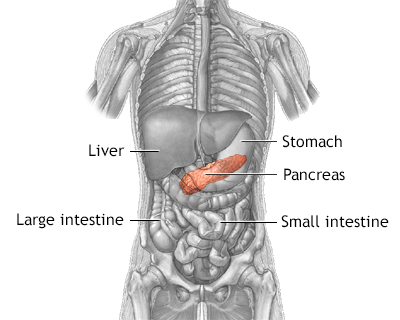
\includegraphics[width=0.5\textwidth]{assets/8883.png}
	\caption{The position of the pancreas in the body and its surrounding organs. Source: \cite{mountsinai_pancreatic_position}.}
	\label{fig:pancreas_position}
\end{figure}

It has 3 main parts, the head lies within the C-shaped curve of the duodenum and the body and tail extend across the midline towards the spleen. \cite{kenhub_pancreas} The division of the pancreas into three main parts (head, body, and tail) helps understand its vascular anatomy too. This is important since radiotracers find their target through this pathways. 

The pancreas receives blood from multiple sources, for example the head gets blood from the superior and inferior pancreaticoduodenal arteries and then drains via the superior mesenteric vein. The suppliers of blood for the body and tail are branches of the splenic artery and drains through the splenic vein. \cite{talathi2023,kenhub_pancreas}

Another relvant part of the pancreas are its ductal system, the main pancreatic duct (Wirsung duct) runs the length of the pancreas and joins with the common bile duct to form the hepatopancreatic ampulla (ampulla of Vater).\cite{kenhub_pancreas} Depicted in figure \ref{fig:pancreas_ducts} as pancreatic duct and Orifice of common bile-duct. 


%where PDAC originates

Pancreatic ductal adenocarcinoma (PDAC) is a highly aggressive malignancy and is characterized by rapid progression. It has distinct biological and structural features, the relevant ones for imaging it are two, altered glucose metabolism (metabolic reprogramming) and a dense fibrotic tumor microenvironment. These characteristics create significant challenges for traditional imaging modalities, thus medical physicists and physicians require advanced techniques like PET/CT for accurate diagnosis.

\begin{figure}[H]
	\centering
	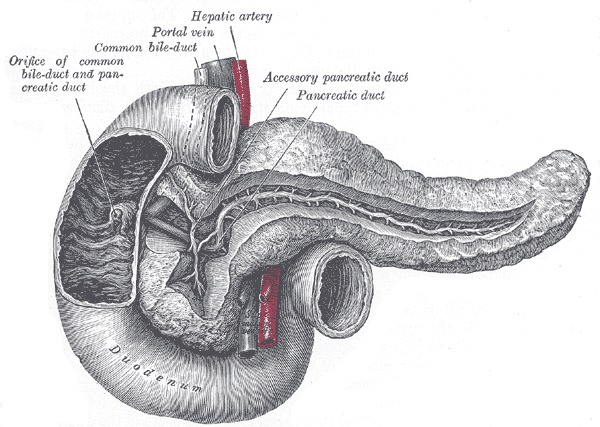
\includegraphics[width=0.5\textwidth]{assets/Gray1100.jpg}
	\caption{The pancreas and its ducts, arteries, and veins. Image by Henry Vandyke Carter, Public Domain, via Wikimedia Commons. Source: \cite{gray_pancreas_ducts}.}
	\label{fig:pancreas_ducts}
\end{figure}

The disease can manifest anywhere in the pancreas but most PDACs (60-70\%) arise from the head. While 20-25\% of PDACs originate in the body or tail of the pancreas. Tumors in the pancreatic head tend to be diagnosed earlier due to their proximity to the common bile duct \cite{stark2015}.

PDAC arises from cells of the pancreatic duct or ductules   \cite{stark2015}. The tumor is often surrounded by a prominent desmoplastic stroma,a dense connective tissue growth, which contributes to its aggressive behavior \cite{haeberle2019}. Because of this, vascular invasion is common, occurring in about 65\% of cases, and is associated with poorer prognosis \cite{hong2012}. Also, as illustrated by figures \ref{fig:pancreas_position} \& \ref{fig:pancreas_ducts} the pancreas has very imporant surrounding structures meaning that PDAC can directly extend into nearby organs like the spleen, adrenals, stomach, and transverse colon. \cite{radiopaedia_pda}

%\subsection{Metabolic Reprogramming in PDAC}

PDAC tumors have metabolic alterations, explained by the Warburg effect.\cite{Hammond2024} The Warbug effect occurs when cells change to a sugar-based energy pathway, over oxygen-based ATP production, even in oxygen-rich conditions. ATP, the molecule cells use for energy, is normally generated through oxygen-driven processes, but glycolysis allows tumor cells to grow rapidly. This shift is driven by genetic mutations associated with cancer, such as KRAS, which increase the production of glucose transport proteins (GLUT1) and processing enzymes (hexokinase-2), this allows for cell proliferation and growth. \cite{Pubmed30721664, Pu2021}.

%what does the images must reveal?

PET/CT imaging for pancreatic lesions must reveal several key features to aid in diagnosis. First, from PET images elevated FDG uptake compared to benign lesions is expected, as cancer cells typically exhibit increased glucose metabolism. This scanner can detect the accumulated hyperglycolytic tumor cells, via the radiotracer [18F]FDG, a glucose analog, meaning it can detect PDAC lesions, with sensitivity rates of 89–91\% and specificity rates of 70–72\% in clinical applications \cite{Pu2021}.

The scan needs to provide information on the size and location of the lesion, as well as any presence of cystic necrosis, since is more common in PDAC (59.6\% of cases). Some other important infomation that can be extracted from a PET/CT scan is the spread of the disease, via vascular invasion or metastases on liver or peritoneal \cite{parikh2020fdg}.  

%how does CT help?
In the past, a conventional PET/CT protocol established that CT scan is perfomed without any alteration. From this scan, data on the attenuation coefficients are obtained and it alows to correct PET images later. It also provides anatomical localisation, so the high FDG part can be identified \cite{benamor2007petct}. Recent studies explore newer and emerging techonology that is used to diagnose PDAC, that include contrast enhanced CT and MRI with Diffusion weight imaging (DWI) and Dynamic Contrast Enhance (DCE), elastography and nanoparticles. \cite{Cancers2023}

% differences with pancreatitis

A main challenge for diagnostics from these images is differentiating PDAC from pancreatitis. The tumor size in mass-forming chronic pancreatitis (MFCP) tends to be larger (mean size $4.00 \pm 0.47$ cm) compared to PDAC (mean size $3.42 \pm 0.75$ cm) \cite{arnone2020}. But those values are pretty close to eachother pointing that diagnosing out of only tumor size is nearly impossible. 

Thankfully, we got some other data to help distinguish between the two. An example is that, PET/CT can better detect vascular invasion, which is more common in PDAC (53.2\%) than in MFCP (23.8\%). And other factors like cystic necrosis and atrophy can also play a role, since these factors and More frequently observed in PDAC than in MFCP \cite{arnone2020}. 

A key factor is that PDAC typically shows higher FDG uptake (higher SUVmax) compared to MFCP due to increased glucose metabolism in cancer cells \cite{arnone2020,Pu2021}. However, even with this metrics diagnostics is quite challenging, as we will explore in a later section on this paper.


%\subsection{Tumor Microenvironment and Imaging Challenges}

Thick fibrous tissue (desmoplastic stroma) surrounds cells in organs, is made up of fibroblast cells and extracellular proteins like collagen. In normal tissues, it provides structure and helps supply nutrients to healthy cells. However, in cancer the stroma becomes abnormally dense and fibrotic. This is called desmoplasia and helps the tumor grow and evade immune attacks, for imaging purposes, this thick tissue also makes it harder for CT and MRI to clearly identify the tumor's boundaries \cite{NCCNGuidelines}.


Additionally, hypoxic regions within the tumor alter glucose metabolism, causing variability in [18F]FDG uptake. This will be discussed in depth later in this document. Making imaging more complicated, inflammatory conditions, such as pancreatitis can produce lesions with overlapping metabolic signatures on PET/CT. As noted by Pu, Y. \cite{Pu2021}, ``both autoimmune pancreatitis and pancreatic cancer appear as metabolic abnormalities and increased FDG accumulation''.


%\subsection{Advanced Imaging Needs}

The challenges presented above highlight the need of development on advanced imaging modalities to ensure accurate diagnosis and staging of these types of cancer. PET/CT combines the sensitivity of metabolic imaging with the spatial resolution of CT, and has emerged as a strong candidate for precise tumor localization and characterization.

Recent studies agree on this and are doing research on the topic. Stating that "The combination of PET and CT can determine the metabolic capacity and anatomical position of pancreatic tumor cells in the body and can accurately diagnose the patient's condition and tumor location" \cite{Pu2021}. Other research shows interest in different modalities, such as PET/MR and the use of other radiotracers for targeting hypoxic or stromal regions. But they all agree that development is needed. This development hold promise for enhancement in diagnostic specificity and sensitivity, although they require validation in clinical settings \cite{Cancers2023}. 

%What could MR offer?

For comparative analysis on PET/MR and PET/CT in therapeutic applications, see also \cite{myownotherpaper}. Where an exploration on what MR offers is included. The main advantages that MRI can add are reduced dose when compared with PET/CT and as an standalone modality, the DWI \& DCE that allows for additional functional information on the ducts and veins of the accesory digestive system organs to be obtained.  
Although both modalities are equivalent in early detection and characterisation, MRI is preferable to CT for imaging surveillance of cystic lesions, particularly in young patients because of cumulative deleterious effects of ionizing radiation with CT \cite{Cancers2023}.


\subsection{The Importance of Early Detection}

Patient outcomes depend entirely on the capacity to early detect pancreatic ductal adenocarcinoma (PDAC). Despite advancements in therapeutic strategies, over 80\% of PDAC patients have locally advanced or metastatic disease at the time of diagnosis, at this stage the curative options are limited. Early-stage detection allows for timely surgical resection, the only potentially curative treatment that improves survival rates \cite{Cancers2023}. 

Because fo the asymptomatic progression and aggressive nature of PDAC its early detection is extraordinarily difficult. Current technology and traditional imaging techniques, like CT and MRI, offer insights when assessing this disease but are limited by heir ability to identify small lesions or distinguish benign from malignant tumors early on. This cases are well illustrated in resource-limited settings, if PET/CT is scarce this challenge becomes even more daunting. For instance, in Mexico PET scanners are centralized in major cities and early detection relies heavily on less sensitive modalities like CT or X-ray, which are often insufficient for timely diagnosis.

The reality of this worldwide problem is showcased in many real-world cases, a personal example is that of my grandmother, whose diagnosis of PDAC came only after her passing, despite months of observation and testing.

Better imaging modalities, such as [18F]FDG-PET/CT, can address some of these issues. The combination of functional and anatomical imaging improves sensitivity and specificity for early lesions, thus enables metabolic changes to be detected before morphological alterations appear \cite{Pu2021}. However, access to these technologies remains uneven globally. As of 2021, Mexico had only 26 PET scanners for its entire population, around 126 Million people \cite{inegi_population}, concentrated in a few hospitals in major cities \cite{statista1}. There is a need for international collaboration to expand access to advanced imaging technologies, both through equipment and expertise.


Another proposed solution to these problems is the addition of surveillance for high-risk groups, with population-specific screening programs targeted to individuals with familial predisposition, cystic lesions, or diabetes mellitus in order to identify precursor lesions or early-stage PDAC \cite{Cancers2023}.

Furthermore, these programs are limited in settings where resources are lacking. Following my personal story, that of my grandmother, who was a high-risk patient with diabetes and a delayed diagnosis, exemplifies the need for accessible and standardized surveillance protocols. The value of those programs not only relies on saving lives but on valuable insights into familial risk factors, which is an area of interest for researchers and patients alike.

When PDAC is diagnosed at a localized stage, surgical resection is more likely to be feasible. Advanced imaging techniques like [18F]FDG-PET/CT offer the potential to identify tumors earlier. Expanding access to these technologies and implementing population-specific screening programs puts the world in the right direction to address this global health challenge and improve outcomes for future patients.
